The \emph{ed-localization}\footnote{\url{https://github.com/tue-robotics/ed_localization}} plugin implements \acrshort{amcl} based on a 2D render from the central world model. In order to navigate, a model of the environment is required. This model is stored in the \acrshort{ed}. From this model, a planning representation is derived that enables using the model of the environment for navigation purposes.
\\
With use of the \emph{ed\_navigation} plugin\footnote{\url{https://github.com/tue-robotics/ed_navigation}}, an occupancy grid is derived from the world model and published as a nav\_msgs/OccupancyGrid. This grid can be used by a motion planner to perform searches in the configuration space of the robot.
\\
With the use of the \emph{cb\_base\_navigation} ROS package\footnote{\url{https://github.com/tue-robotics/cb_base_navigation}} the robots are able to deal with end goal constraints. With use of a ROS service, provided by the ed\_navigation plugin, an end goal constraint can be constructed w.r.t. a specific world model entity described by ED. This enables the robot to not only navigate to poses but also to areas or entities in the scene.
% as illustrated by Figure \ref{fig:ed_navigation_constraints}.
Somewhat modified versions of the local and global ROS planners available within move\_base are used.
%\begin{figure}[h]
%	\centering
%	%\vspace{-0.2cm}
%	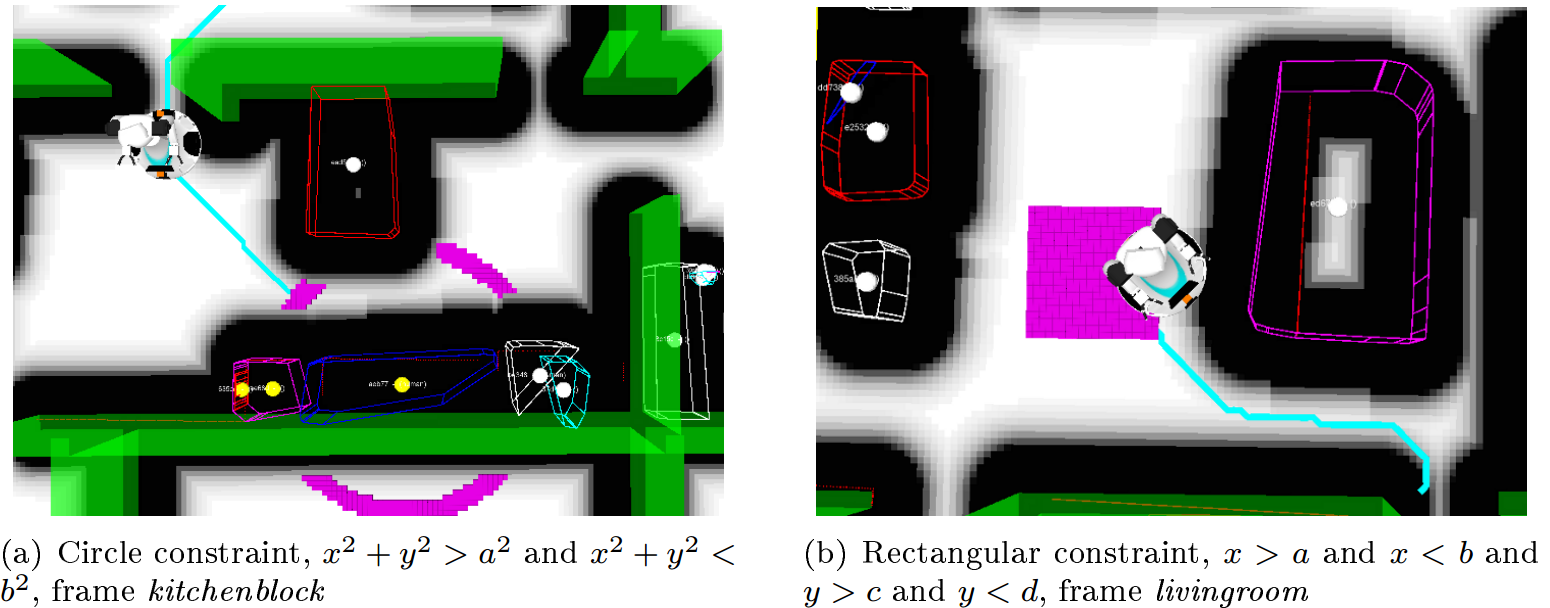
\includegraphics[width = 1\linewidth]{Figures/ed_navigation_constraints}
%	%\vspace{-0.5em}
%	\caption{Navigation position constraints w.r.t. other entities in the environment}
%	\label{fig:ed_navigation_constraints}
%	%\vspace{-0.5cm}
%\end{figure} 